En este capítulo damos algunas definiciones necesarias para presentar la
descomposición de gráficas completas en thrackles.
Empezamos estableciendo conceptos relacionados con gráficas abstractas y después
hablaremos de gráficas en el plano, explicamos el concepto de tipo de orden y cómo
se utiliza en este trabajo. Finalmente hablaremos del anti-thickness abstracto
y del anti-thickness geométrico.

\section{Gráfica}
El concepto base del cual se desprenden otras definiciones es el de gráfica.
Todas las definiciones que presentamos en esta sección fueron tomadas de~\cite{Chartrand2008}.

Una \emph{gráfica} $G$ está compuesta por un conjunto no vacío $V$ de objetos a los que llamamos \emph{vértices}
y por un conjunto $E$, de parejas de elementos de $V$, a los que llamamos \emph{aristas}. Denotamos
a la arista $e$ compuesta por los vértices $u$ y $v$ como $(u,v)$. Para describir a la gráfica $G$
compuesta por el conjunto $V$ de vértices y el conjunto $E$ de aristas escribimos $G=(V,E)$.
Para referirnos al conjunto de vértices de $G$ escribimos $V(G)$ y para referirnos
al conjunto de aristas de $G$ escribimos $E(G)$. En la figura~\ref{fig:g5vex} presentamos
un ejemplo de una gráfica.

\begin{figure}[t]
  \centering
  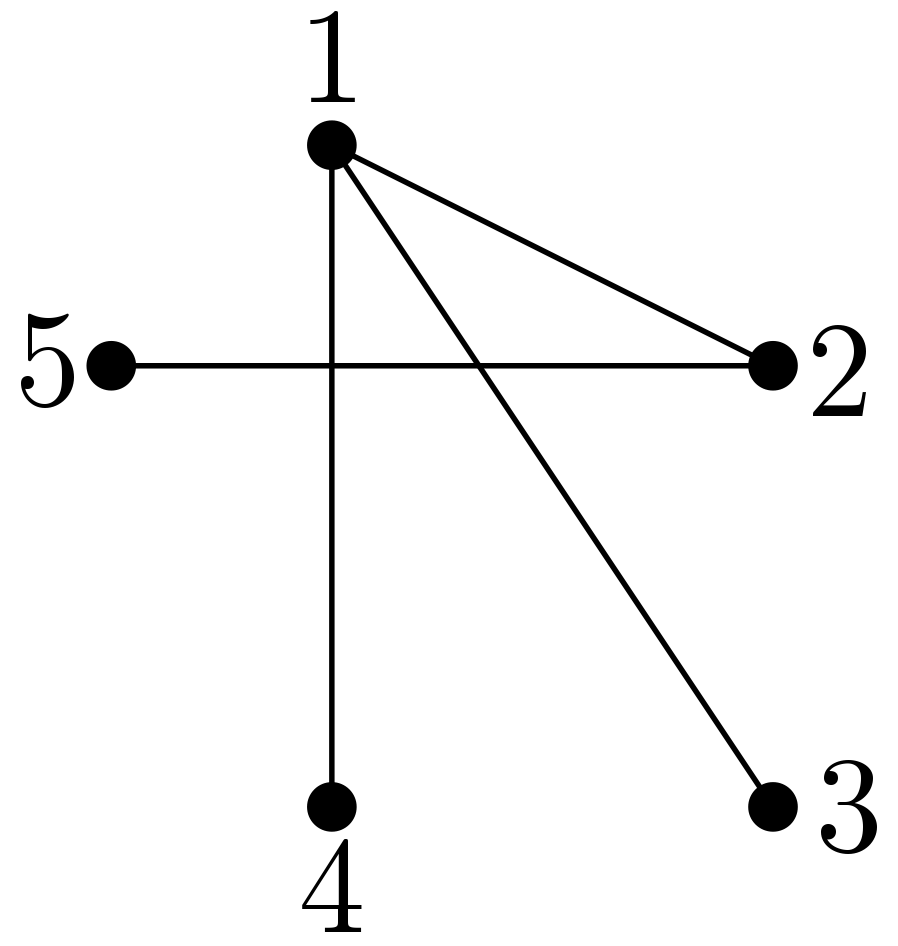
\includegraphics[width=0.3\linewidth]{g5vex.png}
  \caption{Una gráfica de 5 vértices y 4 aristas. Los vértices $1$ y $2$
  son adyacentes y las aristas $(1,3)$ y $(2,5)$ son adyacentes.}
  \label{fig:g5vex}
\end{figure}

Decimos que \emph{dos vértices $u,v\in V(G)$ son adyacentes} si existe la arista
$(u,v)\in E(G)$. La figura~\ref{fig:g5vex} muestra un ejemplo de dos vértices adyacentes.
% \begin{figure}[htb]
%   \centering
%   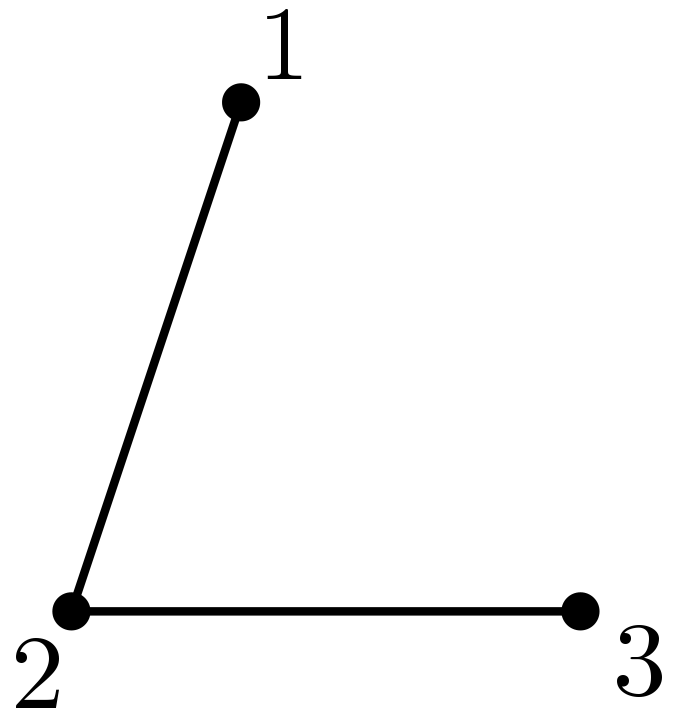
\includegraphics[width=0.3\linewidth]{exady}
%   \caption{En esta gráfica el vértice $1$ es adyacente con el vértice $2$ pero
%   no es adyacente con el vértice $3$.}
%   \label{fig:exady}
% \end{figure}
Decimos que \emph{dos aristas $e_1,e_2 \in E(G)$ son adyacentes}
si inciden en el mismo vértice. Una gráfica es \emph{completa} si cada pareja de vértices
en la gráfica es adyacente. Mostramos un ejemplo de adyacencia de
aristas en la figura~\ref{fig:g5vex} y un ejemplo de una gráfica completa en la figura~\ref{fig:excomplete}.
Para referirnos a la gráfica completa con $n$
vértices escribimos $K_n$. Una gráfica $G$ es \emph{bipartita} si es posible
dar una partición\footnote{Una partición $P$ de un conjunto $X$ es
una colección de subconjuntos que cumplen:
\begin{itemize}
\item Ningún elemento de $P$ es el conjunto vacío.
\item La unión de todos los elementos de $P$ es exactamente el conjunto $X$.
\item La intersección de cualesquiera dos elementos de $P$ es vacía.
\end{itemize} }
de $V(G)$ en dos subcojuntos $U$ y $W$ de tal manera que cada
arista de $G$ tenga un extremo en $U$ y otro extremo en $W$. Presentamos
un ejemplo de gráfica bipartita en la figura~\ref{fig:exbipar}.
\begin{figure}[htb]
  \centering
  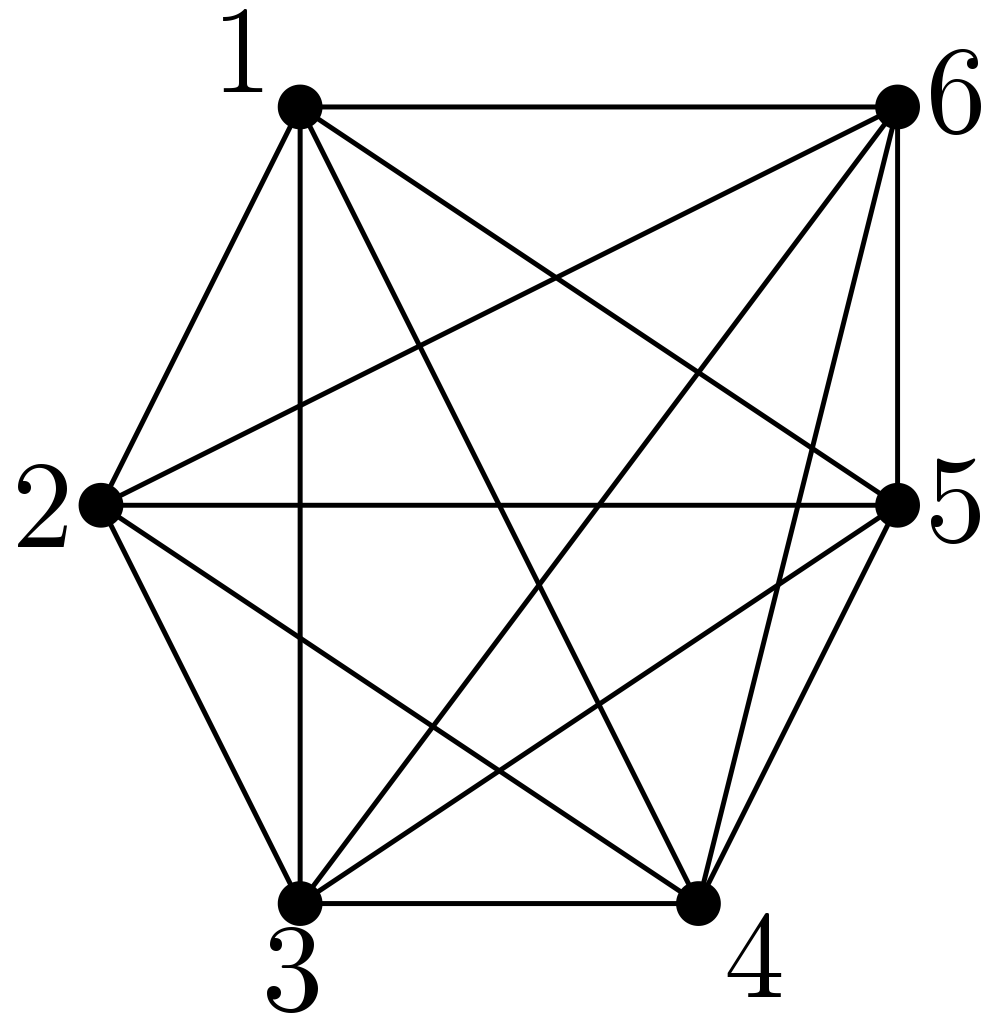
\includegraphics[width=.3\linewidth]{excomplete}
  \caption{La gráfica completa con 6 vértices tiene una arista por cada par de vértices.}
  \label{fig:excomplete}
\end{figure}
\begin{figure}[h]
  \centering
  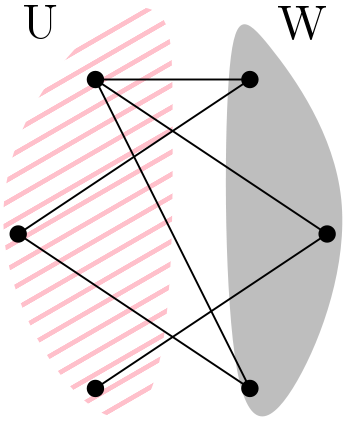
\includegraphics[width=0.3\linewidth]{exbipartita}
  \caption{Un ejemplo de una gráfica bipartita, con conjuntos $U$ y $W$, ambos de tamaño 3.}
  \label{fig:exbipar}
\end{figure}

Una \emph{descomposición} $D$ de una gráfica $G$ es una colección $D=\{G_1,G_2,\dots,G_k\}$ de
subgráficas de $G$ tal que cumple con dos condiciones:
\begin{enumerate}
  \item Ninguna subgráfica $G_i$ contiene vértices aislados.
  \item Cada arista de $G$ pertenece a exactamente una subráfica $G_i$ de $D$.
\end{enumerate}

La figura~\ref{fig:exdecom} ilustra un ejemplo de una descomposición de la gráfica $K_4$.
\begin{figure}[htbp]
  \centering
  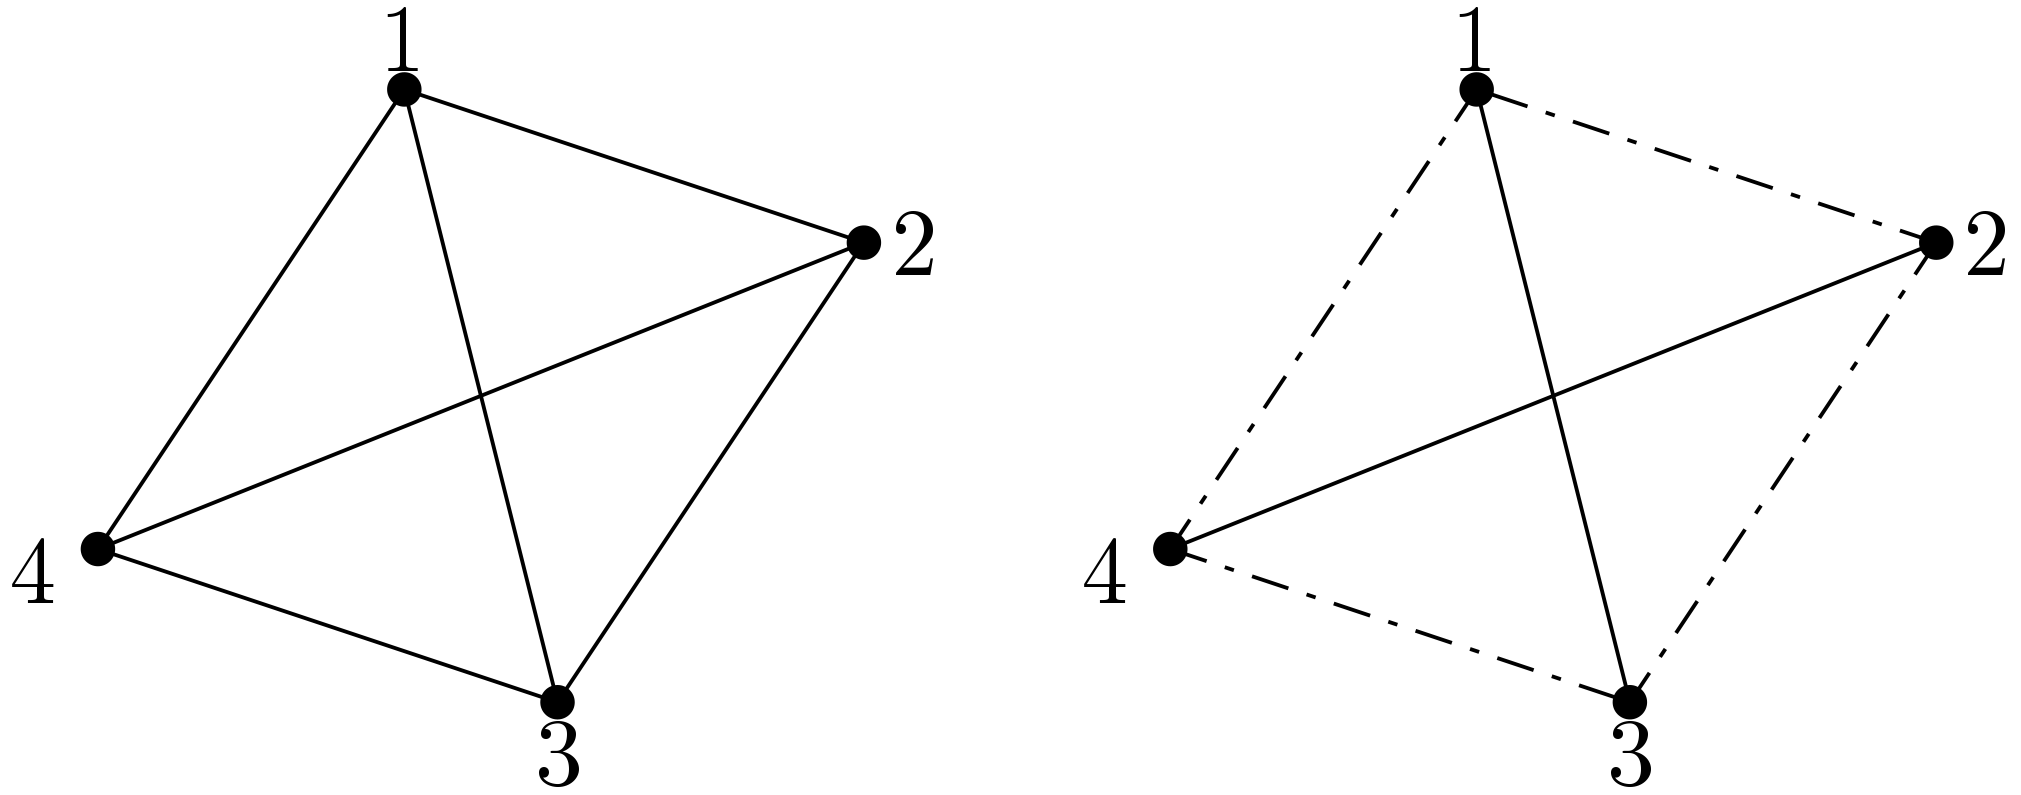
\includegraphics[width=0.7\linewidth]{exdecom}
  \caption{Un ejemplo de una descomposición $D$ de $K_4$ en dos gráficas.
  Aquí $D=\{G_1,G_2\}$ donde $G_1$ es la gráfica compuesta por las aristas $(1,4),(1,2),(2,3),(3,4)$ y
  $G_2$ es la gráfica compuesta por las aristas $(1,3),(2,4)$.}
  \label{fig:exdecom}
\end{figure}
\section{Gráfica geométrica}
Los primeros dos párrafos de esta sección fueron tomados de~\cite{Pach2013}. El tercer párrafo
fue extraido de~\cite{Lara2019}. El cuarto párrafo fue tomado de~\cite{Pach2011}.
Un \emph{dibujo} $\mathsf{G}=(\mathsf{V},\mathsf{E})$ de una gráfica $G$ es una representación de la
gráfica $G$ en el plano tal que 1) cada vértice de $G$ es representado por un punto en el plano
y 2) cada arista de $G$ es representada como una curva simple continua que conecta un par de puntos.
El conjunto de vértices $V$ y el conjunto de aristas $E$ de $\mathsf{G}$
son los puntos y las curvas, respectivamente. Sin perdida de generalidad nos referimos al
conjunto de puntos de $\mathsf{G}$ como $V(\mathsf{G})$, y les llamamos vértices, y nos
referimos al conjunto de curvas de $\mathsf{G}$ como $E(\mathsf{G})$, y les llamamos aristas.

Cuando restringimos las curvas que representan a las aristas del dibujo de $G$
a segmentos de recta llamamos al dibujo de la gráfica como \emph{gráfica geométrica}.
Una gráfica geométrica es completa si existen segmentos de recta entre cada par de vértices
de $V(\mathsf{G})$. En la figura~\ref{fig:exdrawk5} mostramos un dibujo de $K_5$ y una
gráfica geométrica de $K_5$.
\begin{figure}[htpb]
  \centering
  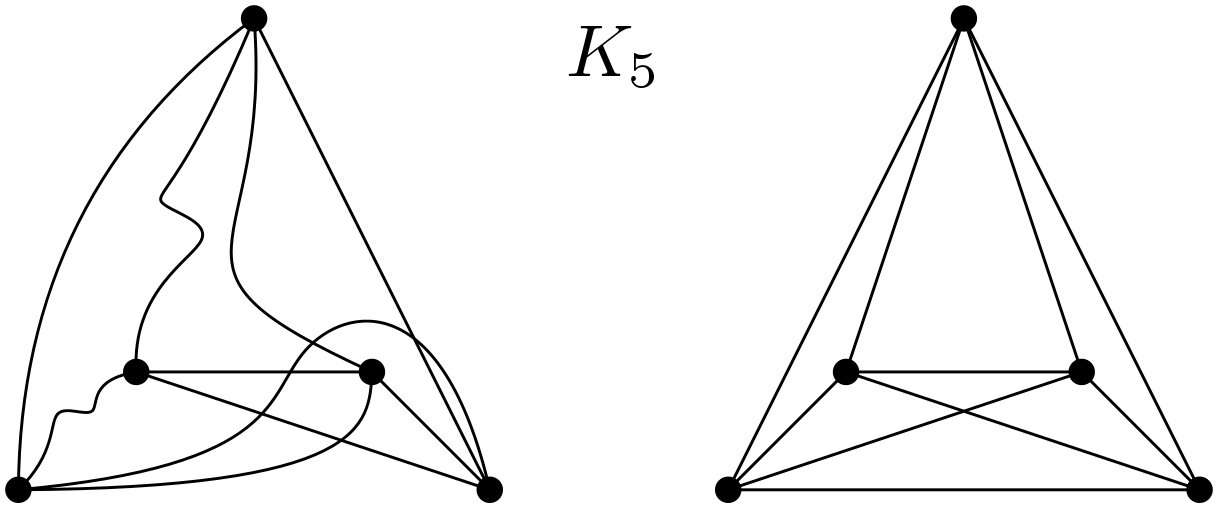
\includegraphics[width=0.8\linewidth]{exdrawk5}
  \caption{A la izquierda observamos un dibujo de $K_5$ y a la derecha observamos
  una gráfica geométrica de $K_5$.}
  \label{fig:exdrawk5}
\end{figure}

Sea $S$ un conjunto de $n$ puntos en posición general en el plano y sea $\mathsf{G}$
una gráfica geométrica de $G$. Decimos que $\mathsf{G}$ está definida sobre $S$ si $V(\mathsf{G}) = S$.
Cualquier conjunto $S$ de puntos en posición general induce una gráfica geométrica completa.

Decimos que dos aristas $e_1,e_2 \in E(\mathsf{G})$ se \emph{cruzan} si existe un punto $p$,
en alguna de las aristas, tal que en $p$ la arista $e_1$ pasa de un lado de la arista
$e_2$ hacia el otro lado. Decimos que dos aristas $e_1, e_2 \in E(\mathsf{G})$ son
\emph{adyacentes} si comparten un vértice.
En este trabajo decimos que dos aristas de una gráfica geométrica se \emph{intersectan}
si son adyacentes o si se cruzan.
Mostramos un ejemplo de intersección de aristas en la figura~\ref{fig:exintersection}.
\begin{figure}[htpb]
  \centering
  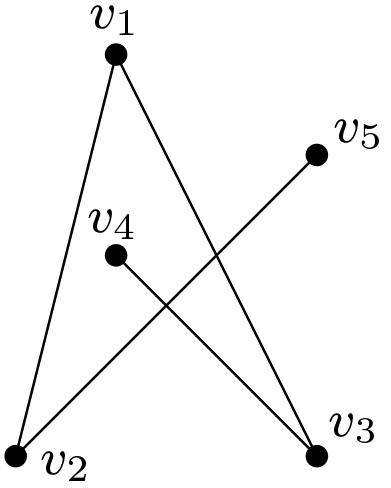
\includegraphics[width=0.3\linewidth]{exintersection}
  \caption{En este ejemplo la arista $(1,2)$ no se intersecta con la arista $(3,4)$
  (son disjuntas) pero sí se intersecta con la arista $(2,5)$.
  La arista $(2,5)$ se cruza con la arista $(3,4)$ y por lo tanto se intersectan.}
  \label{fig:exintersection}
\end{figure}
% Sin perdida de generalidad
% representamos a una gráfica geométrica como $\mathsf{G}$ y nos referimos a su
% conjunto de vértices como $V(\mathsf{G})$ y a su conjunto de aristas como
% $E(\mathsf{G})$.

\section{Thrackles}
Sea $\mathsf{G}$ un dibujo de una gráfica $G$. Decimos que $\mathsf{G}$ es un
\emph{thrackle} si cada par de aristas se intersecta exactamente una vez.
Definidos por John Conway en la decada de 1960, existe una conjetura
que establece que el número de aristas en un thrackle no puede
exceder el número de sus vértices (\cite{brass2006research}).
Un thrackle de $n$ vértices es \emph{máximo} si tiene exactamente
$n$ aristas. La figura~\ref{fig:exmaxth} muestra un thrackle máximo.

\begin{figure}[htpb]
  \centering
  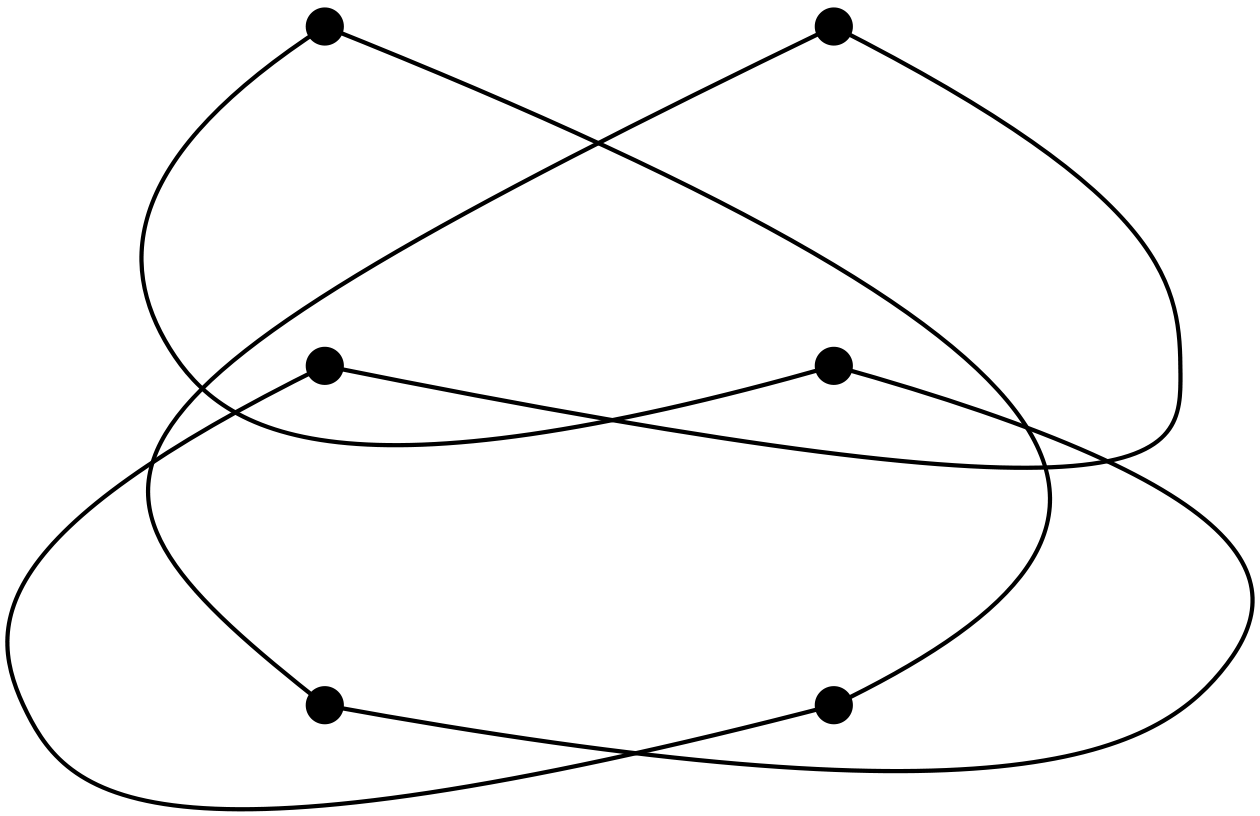
\includegraphics[width=0.35\linewidth]{exmaxth}
  \caption{Un thrackle máximo sobre un conjunto de 6 vértices.}
  \label{fig:exmaxth}
\end{figure}

Un thrackle en el que todas sus aristas son segmentos de recta es conocido como
\emph{thrackle geométrico}(\cite{Schaefer2018}). En este trabajo nos referimos a los thrackles geométricos
como thrackles de manera indistinta. En la figura~\ref{fig:exthgeotop} presentamos un ejemplo de thrackle
y un ejemplo de thrackle geométrico.

\begin{figure}[htb]
  \centering
\begin{subfigure}[h]{.4\textwidth}
  \centering
  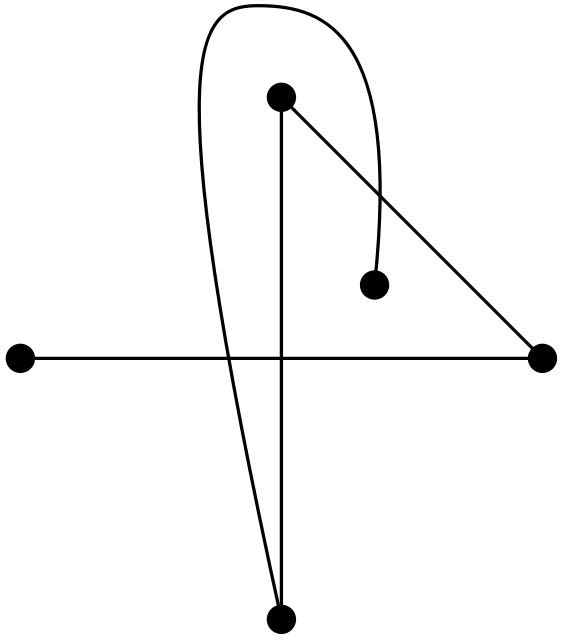
\includegraphics[width=.6\linewidth]{exthtop}
  \caption{Un thrackle de 5 vértices.}
  \label{fig:exthtop}
\end{subfigure}\hfill%
\begin{subfigure}[h]{.4\textwidth}
  \centering
  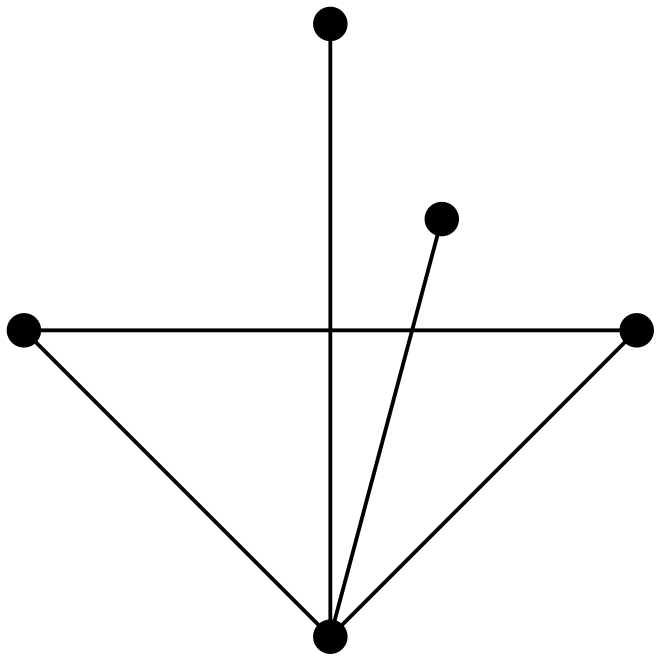
\includegraphics[width=.6\linewidth]{exthgeo}
  \caption{Un thrackle geométrico con 5 vértices.}
  \label{fig:exthgeo}
\end{subfigure}
\caption{Ambas figuras ilustran thracklese definidos sobre el mismo conjunto de
puntos. En los dos casos el thrackle dibujado es máximo.}
\label{fig:exthgeotop}
\end{figure}

Una descomposición por thrackles $D$, de una gráfica geométrica
$\mathsf{G}$, es una colección $D=\{\mathsf{G}_1,\mathsf{G}_2,\dots,\mathsf{G}_k\}$
de subgráficas que cumple con tres condiciones:
\begin{enumerate}
  \item Cada subgráfica $\mathsf{G}_i$ es un thrackle.
  \item Ninguna subgráfica $\mathsf{G}_i$ contiene vértices aislados.
  \item Cada arista de $\mathsf{G}$ pertenece a exactamente una subráfica $\mathsf{G}_i$ de $D$.
\end{enumerate}

Una gráfica (abstracta) $G$ es \emph{thrackleable} si puede ser dibujada en el plano como un thrackle.
\section{Tipo de Orden}
Las definiciones de esta sección fueron tomadas de~\cite{Aichholzer2002}.
El tipo de orden de un conjunto $S$ de $n$ puntos en posición general, digamos
$S=\{p_1,p_2,\dots,p_n\}$ es una función que asigna a cada tripleta ordenada
$i,j,k \in \{1,2,\dots,n\}$ la orientación de la tripleta de puntos $\{p_i,p_j,p_k\}$\footnote{
Tres puntos en el plano en posición general pueden tener una orientación en sentido horario
o una orientación en sentido anti-horario.}. En la figura X mostramos un ejemplo de
cada orientación posible para una tripleta.
Decimos que dos conjuntos $S_1$ y $S_2$ son \emph{combinatoriamente equivalentes} si
tienen el mismo tipo de orden. En la figura~\ref{fig:exotk5} presentamos conjuntos
combinatoriamente equivalentes de 5 puntos. En la figura~\ref{fig:ot5}
mostramos los diferentes tipos de orden para un conjunto de 5 puntos.

\begin{figure}[htpb]
  \centering
  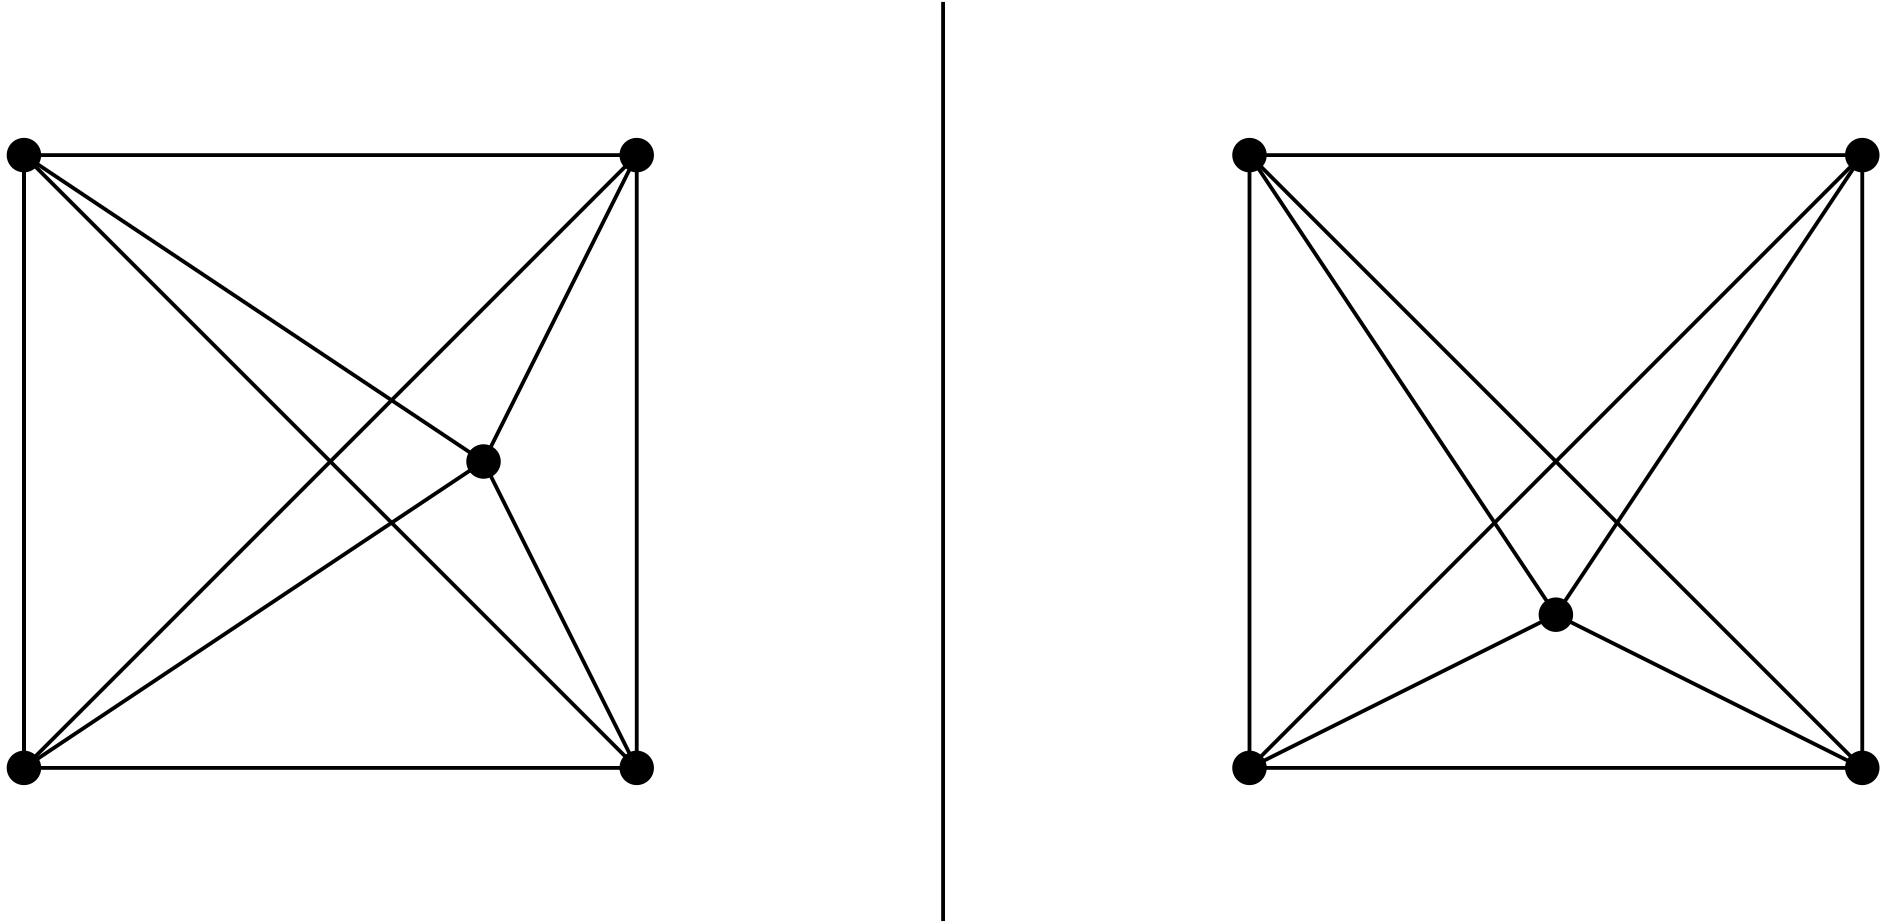
\includegraphics[width=0.6\linewidth]{exotk5}
  \caption{Estos dos conjuntos de puntos tienen el mismo tipo de orden.}
  \label{fig:exotk5}
\end{figure}
\begin{figure}[htpb]
  \centering
  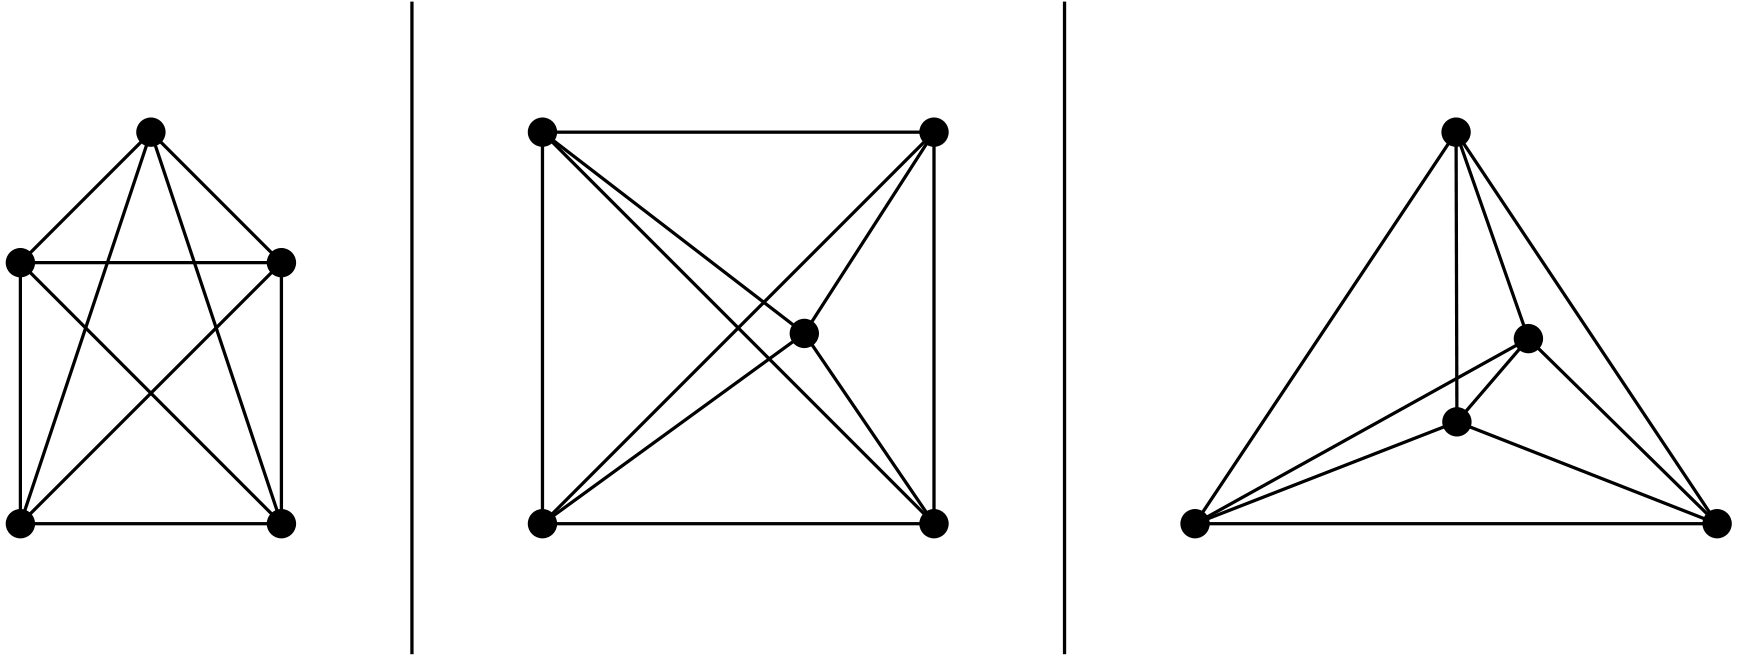
\includegraphics[width=0.8\linewidth]{ot5}
  \caption{Las tres maneras diferentes de distribuir 5 puntos en el plano. Cualquier
  otra configuración es equivalente a alguna de estas tres configuraciones.}
  \label{fig:ot5}
\end{figure}

\section{Anti-thickness y anti-thickness geométrico}
Las siguientes definiciones fueron tomadas de~\cite{Dujmovic2017}.
\begin{definition}{\emph{Anti-thickness de una gráfica.}}
  El anti-thickness de una gráfica $G$ es el entero $k$ más pequeño tal que existe una
  partición de $E(G)$, de tamaño $k$, en la que cada elemento de la partición
  es una gráfica thrackleable.
\end{definition}
La figura~\ref{fig:exantithickness} ilustra un ejemplo del anti-thickness de $K_5$.
\begin{figure}[htpb]
  \centering
  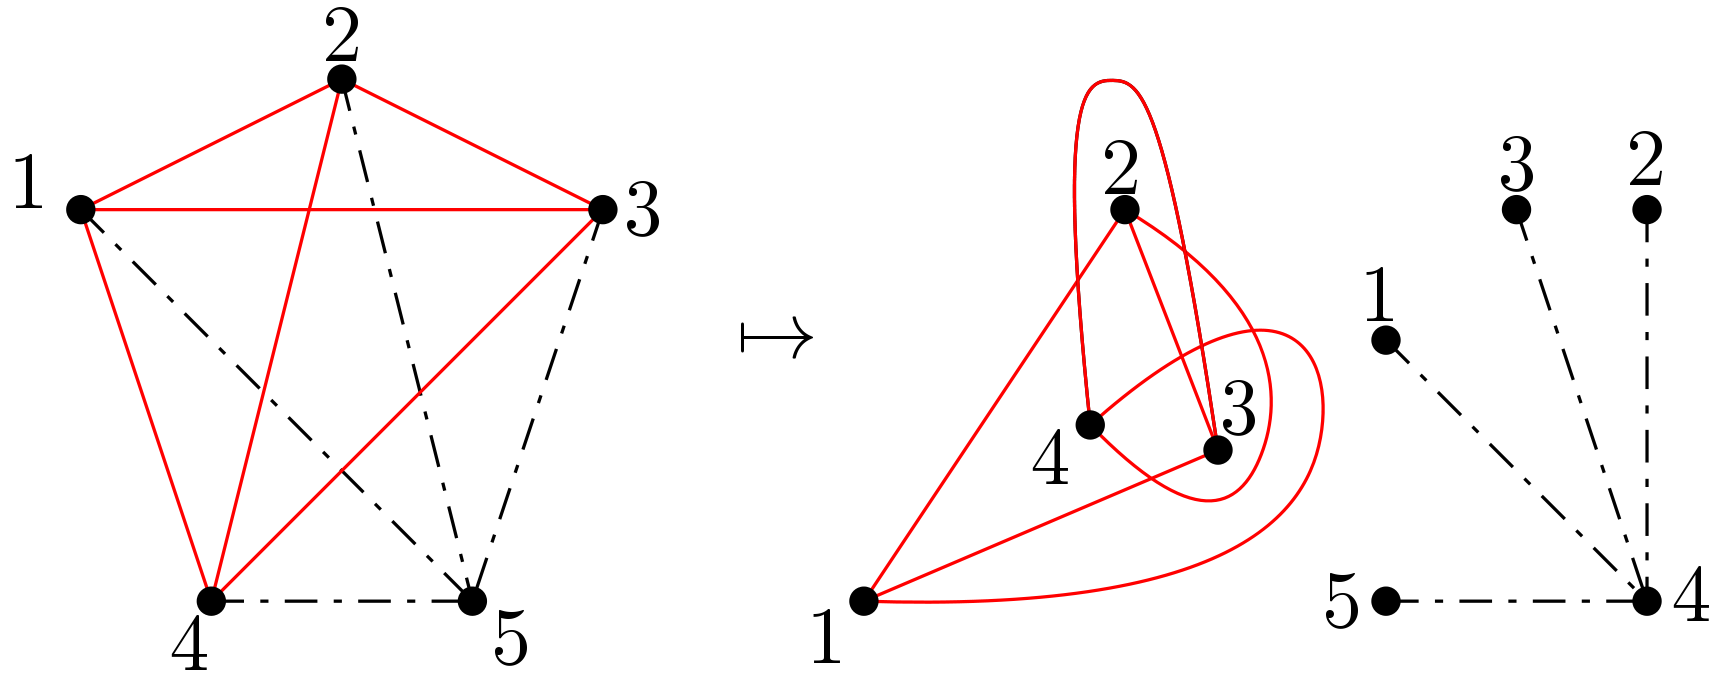
\includegraphics[width=0.7\linewidth]{exantithickness}
  \caption{La figura muestra a $K_5$ a la izquierda y a la derecha dos thrackles
  cuya unión es la gráfica completa. Consideremos las aristas de la gráfica completa inducida por los vértices $1,2,3,4$,
  estas aristas inducen un thrackle mientras que las aristas con un extremo en el vértice $5$ inducen otro thrackle.
  El anti-thickness de $K_5$ es precisamente igual a dos ya que si fuera uno la gráfica $K_5$ tendría un dibujo
  que es un thrackle y esto no es posible.}
  \label{fig:exantithickness}
\end{figure}
\begin{definition}{\emph{Anti-thickness geométrico de una gráfica.}}
El anti-thickness geométrico de una gráfica $G$ es el entero $k$ más pequeño tal que
existe un dibujo $\mathsf{G}$ de $G$ para el cual hay una partición de $E(\mathsf{G})$,
de tamaño $k$, en la que cada elemento de la partición es un thrackle.
\end{definition}
En la figura~\ref{fig:exantithicknessgeo} damos un ejemplo del anti-thickness geométrico de $K_5$.
\begin{figure}[htpb]
  \centering
  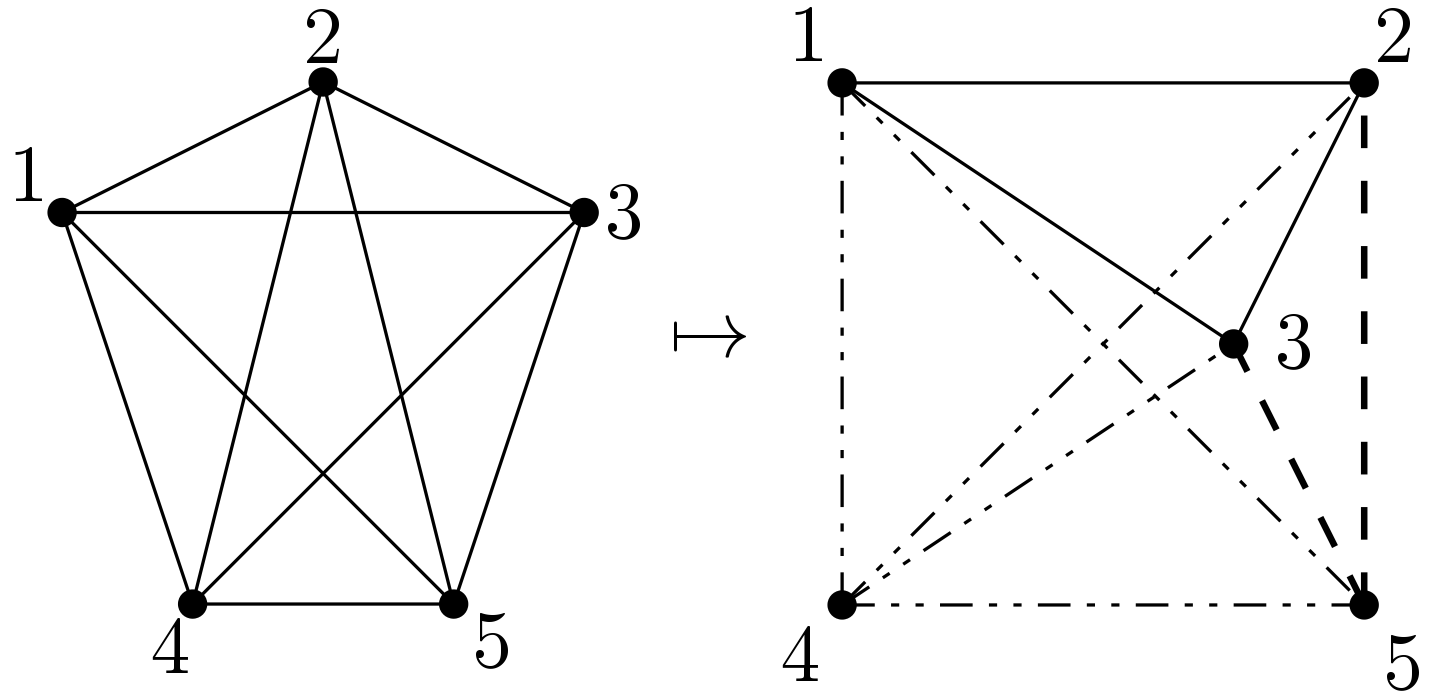
\includegraphics[width=0.6\linewidth]{exantithicknessgeo}
  \caption{En esta figura podemos observar una descomposición de $K_5$ en 3 thrackles
  geométricos. Esta descomposición se muestra en la figura del lado derecho, cada
  thrackle está dibujado con diferentes patrones de línea. El anti-thickness geométrico
  de $K_5$ es exactamente tres, esto es demostrado en la sección de resultados.}
  \label{fig:exantithicknessgeo}
\end{figure}
\section{Número cromático}
Las siguientes definiciones fueron tomadas de~\cite{Chartrand2008}.

Una \emph{coloración propia} de los vértices de una gráfica $G$ es la asignación
de colores a los vértices de $G$ tal que cada vértice tiene un solo color
asignado y dos vértices adyacentes tienen diferentes colores.
Un color puede ser un color como rojo, verde, amarillo, etc. cuando el número
de colores a usar es pequeño, de otra forma se usan enteros $1,2,\dots,k$
para algún entero positivo $k$. Si asignamos $k$ colores
diferentes de esta manera decimos que tenemos una \emph{k-coloración} de la gráfica $G$.
Dada una $k$-coloración de una gráfica $G$ y sea $V_i$ el conjunto de vértices
de $G$ que tienen el color $i$ asignado. Entonces llamamos a $V_i$
una \emph{clase cromática}. Los elementos de $V_i$ generan una \emph{partición}
de los vértices de $G$.

Una gráfica $G$ es \emph{k-colorable} si existe una coloración propia de $G$ de tamaño $k$.
El entero positivo $k$ más pequeño para el cual $G$ es $k$-colorable recibe el nombre
de \emph{número cromático} de $G$. Lo denotamos como $\chi(G)$.
Si consideramos cualquier partición de $V(G)$, el número cromático $\chi(G)$ de $G$ es la
cardinalidad más pequeña posible de dicha partición.
% El número cromático
% de $G$ es el mínimo número de conjuntos independientes que pueden existir en una partición
% de $V(G)$.

La figura~\ref{fig:excoloring} muestra un ejemplo de una coloración propia de una gráfica $G$.
En este ejemplo ilustramos cada clase cromática dibujando los vértices con diferentes colores
representados por una cruz, un circulo y un cuadrado.
\begin{figure}[htpb]
  \centering
  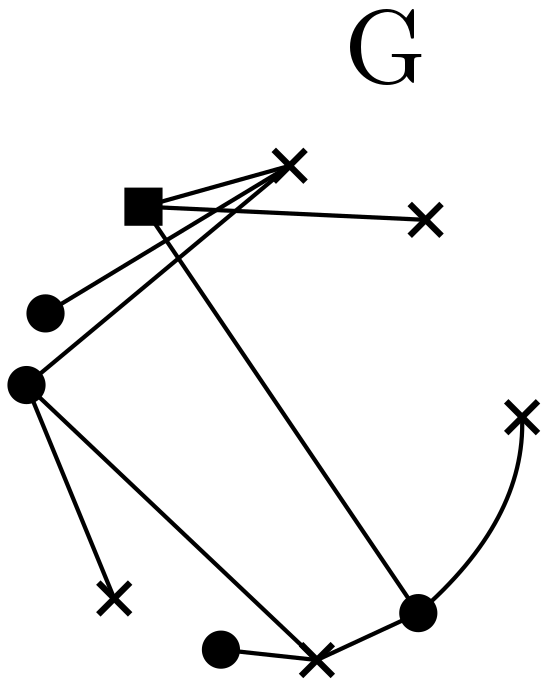
\includegraphics[width=0.35\linewidth]{excoloring}
  \caption{Una coloración propia de una gráfica $G$. Esta coloración es de tamaño 3, por
  lo tanto decimos que es una 3-coloración de $G$. Para esta gráfica en particular
  no existe una coloración más pequeña, por lo que su número cromático es 3. Nótese
  que los conjuntos independientes son formados por vértices que tienen el mismo
  color asignado y no son adyacentes entre sí.}
  \label{fig:excoloring}
\end{figure}
